\begin{figure}[tp]
    \begin{minipage}[h]{0.5\linewidth}
    \center{
        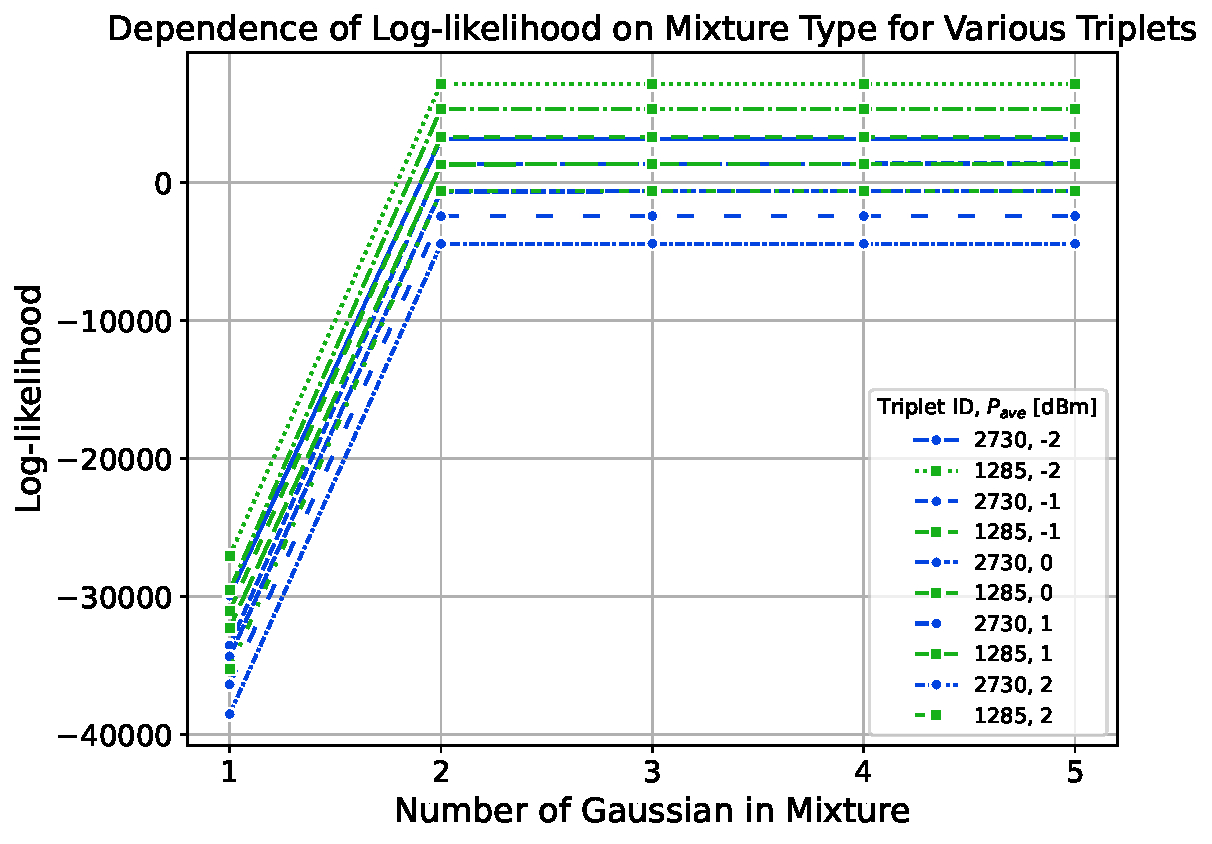
\includegraphics[width=1\linewidth]{images/gauss/bigf_loglik_vs_mixture_low.pdf} (a) \\
    }
    \end{minipage}
    \begin{minipage}[h]{0.5\linewidth}
    \center{
        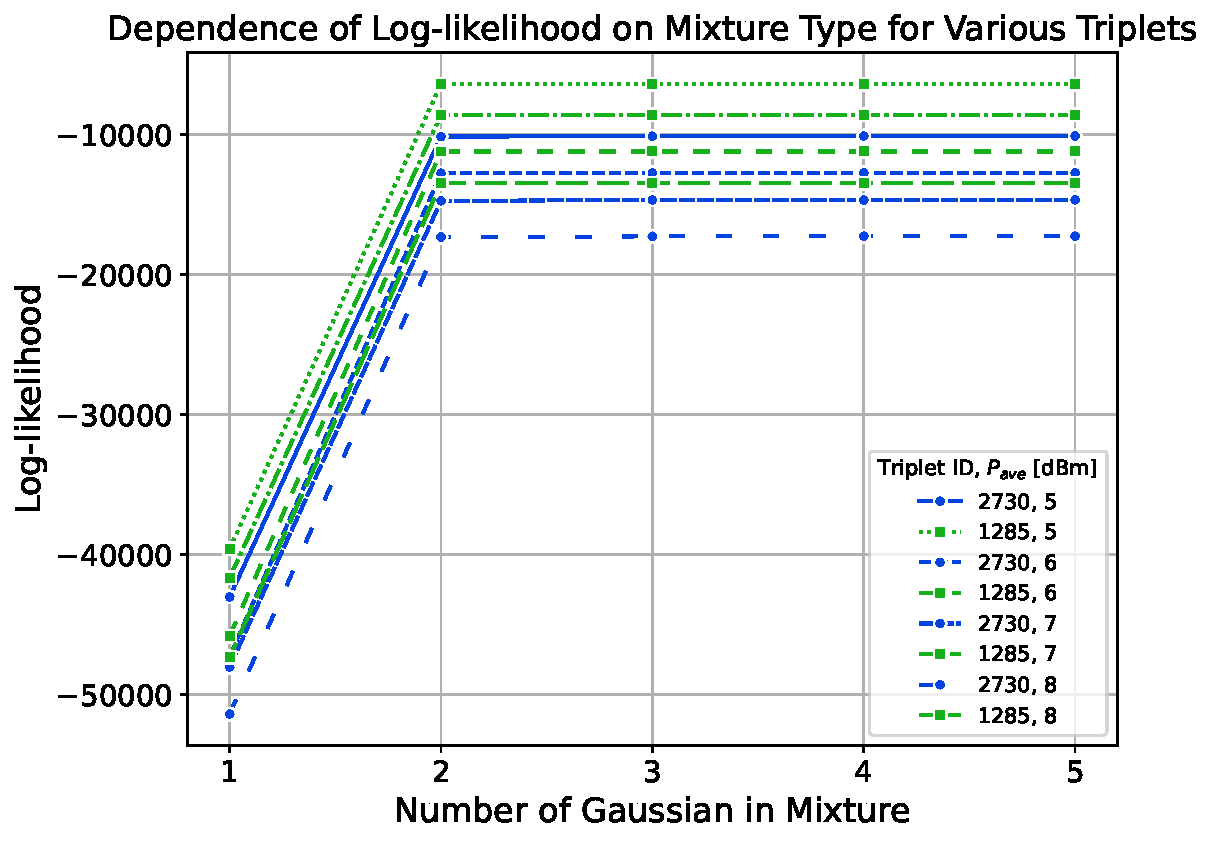
\includegraphics[width=1\linewidth]{images/gauss/bigf_loglik_vs_mixture_high.pdf} (b)\\
    }
    \end{minipage}

    \caption{Log-likelihood dependence for triplet distribution for different number of components in \gls{gmm}. Graph shows triplets with ID 2730 $[3+3\mathrm{i}, 3+3\mathrm{i}, 3+3\mathrm{i}]$ and ID 1285 $[-1-1\mathrm{i}, 1+1\mathrm{i}, -1-1\mathrm{i})]$.}
    \label{fig:lines_different_mix}
\end{figure}